
%%%%%%%%%%%%%%%%%%%%%%%%%%%%%%%%%%%%%%%%%%%%%%%%%%%%%%%%%%%%%%%%%%%%%%%%%
%           Capítulo 3: NOMBRE                   %
%%%%%%%%%%%%%%%%%%%%%%%%%%%%%%%%%%%%%%%%%%%%%%%%%%%%%%%%%%%%%%%%%%%%%%%%%

\chapter{Diseño del experimento}
En este capítulo, se presenta la introducción al desarrollo de la tesis, ya sea el modelo matemático o las bases del proyecto, etc.
Ejemplo de cita  [\citet{latex}]
Ejemplo de cita [\citeauthor{RR73}]
 % The \cite command functions as follows:
 %   \citet{key} ==>>                Jones et al. (1990)
 %   \citet*{key} ==>>               Jones, Baker, and Smith (1990)
 %   \citep{key} ==>>                (Jones et al., 1990)
 %   \citep*{key} ==>>               (Jones, Baker, and Smith, 1990)
 %   \citep[chap. 2]{key} ==>>       (Jones et al., 1990, chap. 2)
 %   \citep[e.g.][]{key} ==>>        (e.g. Jones et al., 1990)
 %   \citep[e.g.][p. 32]{key} ==>>   (e.g. Jones et al., p. 32)
 %   \citeauthor{key} ==>>           Jones et al.
 %   \citeauthor*{key} ==>>          Jones, Baker, and Smith
 %   \citeyear{key} ==>>             1990





%%%%%%%%%%%%%%%%%%%%%%%%%%%%%%%%%%%%%%%%%%%%%%%%%%%%%%%%%%%%%%%%%%%%%%%%%
%                          Descripción de la planta                     %
%%%%%%%%%%%%%%%%%%%%%%%%%%%%%%%%%%%%%%%%%%%%%%%%%%%%%%%%%%%%%%%%%%%%%%%%%
\section{Sección}
El sistema blah, blah. Ejemplo de cita \citep{texbook}
La figura (\ref{planta})                     %hace referencia a la imagen "planta" el número se inserta automáticamente
 ilustra los componentes de la planta.

\begin{figure}
  \centering
    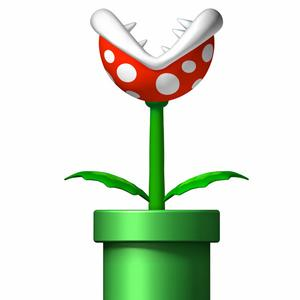
\includegraphics[scale=0.5]{Capitulo3/figs/planta.jpg}      %Ruta completa de la imagen, porque se compila desde el archivo tesis.tex
  \caption{Descripción de la planta}            %Pie de imagen
  \label{planta}                            %nombre de referencia
\end{figure}




%%%%%%%%%%%%%%%%%%%%%%%%%%%%%%%%%%%%%%%%%%%%%%%%%%%%%%%%%%%%%%%%%%%%%%%%%
%                          Modelado                                     %
%%%%%%%%%%%%%%%%%%%%%%%%%%%%%%%%%%%%%%%%%%%%%%%%%%%%%%%%%%%%%%%%%%%%%%%%%
\section{\textcolor{Azul}{Sección en color azul}}
\subsection{Subsección}
Antes de comenzar, se definen  en la tabla ~\ref{tab:tabla} los parámetros y variables utilizadas

%%%%%%%%Tabla Nombres de parámetros
\begin{table}[ht]                             %Inicia el entorno table debajo del texto
\centering\                                     %   centra la tabla
\begin{tabular}{||c | c ||}                     %inicia entorno tabular con doble línea en las orillas, 2 columnas con el contenido centrado (c)
\hline                                          %inserta línea horizontal
\hline
Nombre Parámetro/Variable & Símbolo\\
\hline
\hline
Masa del péndulo & $m$ \\
\hline
Masa del carro & $M$\\
\hline
Distancia del eje de giro al centro de masa & $l$ \\
\hline
Aceleración gravitatoria & $g$ \\
\hline
Momento de inercia péndulo respecto del eje de giro& $J$ \\
\hline
Ángulo del péndulo respecto del eje vertical & $\theta$\\
\hline
Velocidad angular del péndulo & $\dot{\theta}$, $\omega$\\
\hline
Distancia del carro respecto al centro del riel & x\\
\hline
Velocidad del carro & $\dot{x}$, $v$\\
\hline
\hline
\end{tabular}
\caption[Parámetros dinámicos del carro-péndulo]{\textbf{Parámetros dinámicos del carro-péndulo} - Estos son los valores de parámetros utilizados en el diseño y las simulaciones, corresponden a los valores reales.}
\label{tab:tabla}                              %etiqueta para referencia
\end{table}

\blindtext


%%%%%%%%%%%%%%%%%%%%%%%%%%%%%%%%%%%%%%%%%%%%%%%%%%%%%%%%%%%%%%%%%%%%%%%%%
%                          Subsección
%%%%%%%%%%%%%%%%%%%%%%%%%%%%%%%%%%%%%%%%%%%%%%%%%%%%%%%%%%%%%%%%%%%%%%%%%

\subsection{Otra subsección}

\Blindtext